\chapter{معماری نمونه مطالعاتی برنامه اشتراک سفر}

\section{زمینه برنامه اشتراک سفر}
هدف ایجاد یک بازار برخط میان رانندگان و مسافران است تا از یک سمت نیاز مسافران برای یافتن رانندگانی که مقاصد و شرایط نزدیک به دلخواه آن برای سفر دارند رفع شود و از سوی دیگر رانندگان قادر باشند تا مسافران باب میل خود را از میان مسافرین انتخاب کنند.در این میان برنامه باید اطلاعات سفر ها را لحظه به لحظه رصد کند تا از بروز هر گونه مشکل جلوگیری شود.

معماری پیشنهادی برای چنین زمینه\LTRfootnote{Context} ای معماری \lr{micro-service} است تا با شکستن برنامه بر اساس عملکرد‌ها\LTRfootnote{Functionalities} به میکرو سرویس های متناظر، نیازهای کیفی و غیرکیفی را مرتفع سازد.به این صورت با شکستن برنامه به مولفه‌های تقریبا مستقل بر حسب منطق تجاری به برنامه قابلیت حمل، انعطاف‌پذیری، رشد و گسترش‌پذیری بیشتری داده می‌شود.

در مورد بحث دردسترس‌پذیری در معماری میکروسرویس، تاب‌‌آوری\LTRfootnote{Resilience} مهم‌ترین فاکتور است؛ حفظ دسترس‌پذیری با مدیریت و مانیتورینگ صحیح سرویس‌ها امکان‌پذیر خواهد بود.گسترش‌پذیری در معماری میکروسرویس در گرو تخصیص بهینه منابع به سرویس ها توسط مولفه توزیع‌بار\LTRfootnote{LoadBalancer} است.

\section{معماری پیشنهادی}

الگو معماری میکرو‌سرویس‌ها روشی برای توسعه برنامه در قالب سرویس‌های کوچک است که هر کدام به صورت تقریبا مستقل فعالیت می‌کنند.این الگو امکان تحویل/استقرار مداوم\LTRfootnote{Continouse Delivery/Development} برنامه های پیچیده و بزرگ را فراهم می کند و همچنین به یک سازمان امکان می دهد تا به تدریج پشته فناوری خود را توسعه دهد.
\begin{figure}[h]
\centering
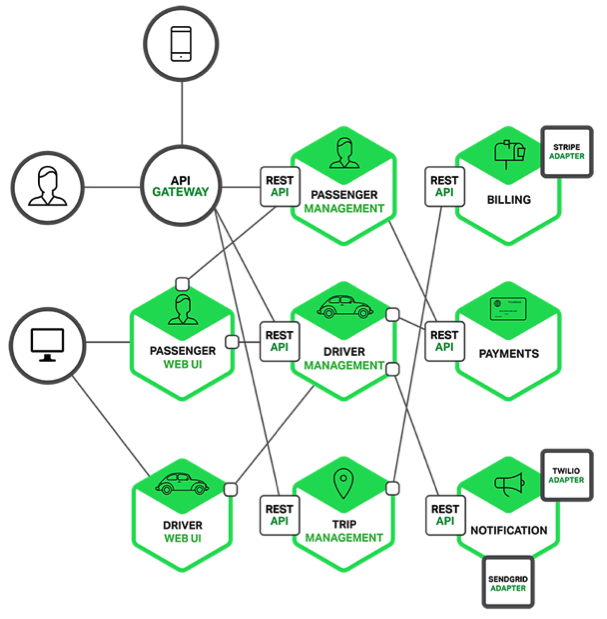
\includegraphics[scale=0.7]{trip.png}
\caption{معماری میکروسرویس برنامه اشتراک سفر}
\label{fig:trip}
\end{figure}


\section{نیازمندی‌های پوشش‌داده شده توسط معماری}
در ادامه به تجزیه و تحلیل مشخصات معماری رایج برای الگوی معماری میکرو‌سرویس ها و میزان توانایی این الگو در رفع نیاز‌های کیفی پرداخته می‌شود.

چابکی و توانایی پاسخ سریع به تغییرات محیطی در کسب‌و‌کار‌های رقابتی نظیر صنعت حمل‌و‌نقل اهمیت بالایی دارد.با توجه به مفهوم واحدهای مستقل و کوچک در الگوی میکرو‌سرویس برنامه با چنین الگویی می‌تواند با کمترین هزینه تغییرات لازم را در خود اعمال کند و از قابلیت تغییر‌پذیری\LTRfootnote{Modifiability} بالایی برخوردار است.

به دلیل تفکیک عملکرد و دغدغه‌های تجاری در برنامه‌ها با الگوی میکرو‌سرویس، می توان تست را محدود کرد، و این امر باعث می شود که آزمایشات هدفمندتر انجام شوند.همچنین آزمون برای یک سرویس خاص بسیار آسان تر و عملی تر از نوشتن آزمون برای یک معماری \lr{Monolithic} است و چون در معماری میکروسرویس مولفه‌ها \lr{lously coupled} هستند امکان این‌که یک تغییر در یک سرویس منجر به شکست سایر سرویس‌ها شود،کم است.

به دلیل ذات توزیع‌شده و نیاز به پیام‌رسانی تحت شبکه در الگوی میکروسرویس نوشتن سرویس‌ها با کارایی بالا در خروجی مناسب بسیار اهمیت دارد و یکی از چالش‌های استفاده از الگوی میکروسرویس حفظ کارایی در هنگام گسترش برنامه است اما در مقابل چالش کارایی گسترش‌پذیری برنامه تحت این الگو به راحتی صورت می‌پذیرد و با ساختار خود پیچیدگی مسائل رو با شکستن به ریز‌سرویس ها کاهش می‌دهد.
























